\Chapter{ゼータ関数(田村)}
%\Section{ゼータ関数(田村)}
\Section{\S 0.はじめに}
ますらぼには数学が好きな高校生も来るということで,なるべく高校生にもわかるよう書いてみた.正則性など細かい条件をごまかしているが,多項式や$e^x$などの高校で出てきた関数の組み合わせなら大体成り立つと思っておけばいい.興味のある人は複素解析の本を読んでみるといいと思う.\\
さて,タイトルのゼータ関数とは
\[
\zeta(s)=\sum_{n=1}^\infty\frac{1}{n^s}=\frac{1}{1^s}+\frac{1}{2^s}+\cdots
\]
という関数で,リーマンの論文「与えられた数よりも小さな素数の個数について」\cite{Riemann}にも現れる重要な関数である.\\
具体的な値を挙げておくと次の通りである.
\begin{eqnarray*}
\zeta(2)=\frac{1}{1^2}+\frac{1}{2^2}+\cdots &=& \frac{\pi^2}{6}\\
\zeta(4)=\frac{1}{1^4}+\frac{1}{2^4}+\cdots &=& \frac{\pi^4}{90}\\
\zeta(6)=\frac{1}{1^6}+\frac{1}{2^6}+\cdots &=& \frac{\pi^6}{945}
\end{eqnarray*}
偶数ゼータに対しては,なぜ$\pi$が出てくるのかは不思議だが,上の様な値になることが知られている.\\
では次の式を見てどう思うだろうか.
\begin{eqnarray*}
\zeta(0)=1+1+\cdots &=& -\frac{1}{2}\\
\zeta(-1)=1+2+\cdots &=& -\frac{1}{12}
\end{eqnarray*}
中辺は明らかに発散する無限和である.それが有限の値になるというのは理解し難い.少しずつその謎を紐解いていこうと思う.

\Section{\S 1.予備知識}
\Subsubsection{初等関数の複素数での値}
オイラーの公式$e^{iz}=\cos z+i\sin z$を用いると
\[
\cos z=\frac{e^{iz}+e^{-iz}}{2}, \sin z=\frac{e^{iz}-e^{-iz}}{2i}
\]
となる.\\
また,絶対値が$r>0$,偏角が$\theta$の複素数は$z=r(\cos\theta+i\sin\theta)=re^{i\theta}$となるので, $z$の対数は
\[
\log z=\log r +i\theta
\]
となる.ただし,偏角は$2\pi$の整数倍だけ異なることができるので, $\log$は一般には多価関数となる.そこで定義域を0と負の実数を除く領域に制限し,偏角を$-\pi<\theta<\pi$とすることで一価に定まる.これを対数関数の主枝と呼ぶ.

\Subsubsection{複素数平面上の積分}
$f(z)$が連続, $\gamma(t)\colon[0,1]\to\mathbb{C}$が区分的$C^1$であれば, $f(z)$の$\gamma$に沿った積分は
\[
\int_\gamma f(z)dz = \int_0^1 f(\gamma(t))\gamma'(t)dt
\]
となる.\\

\begin{wrapfigure}[7]{r}{50mm}
\vspace{-2\baselineskip}
\begin{center}
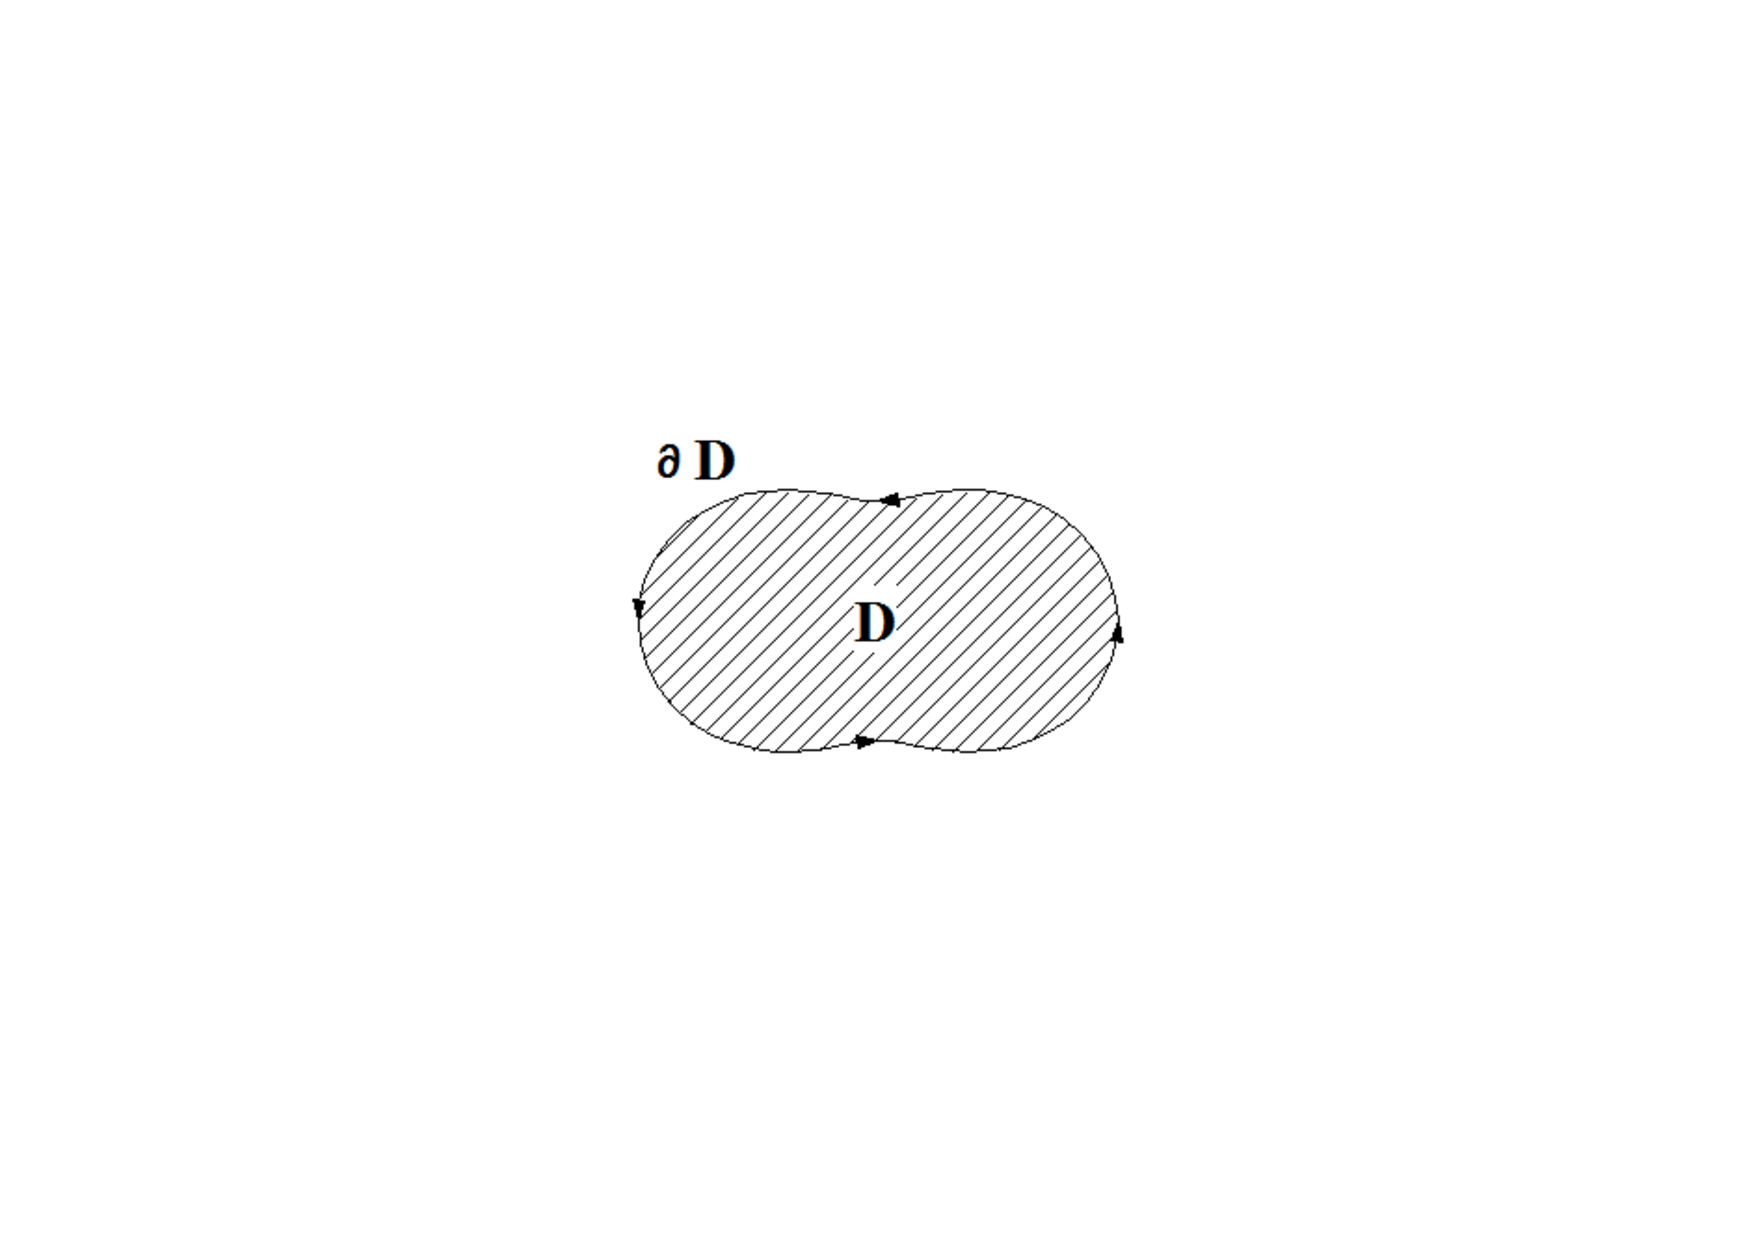
\includegraphics[width=50mm]{zetamura1.pdf}
\end{center}
\end{wrapfigure}
$D$を複素数平面上の区分的$C^1$の境界をもつ領域とし, $\partial D$を$D$の境界で$D$を左手に見て進む向きをもつ閉曲線とする.このとき次の公式が成り立つ.\\
$s\in \mathbb{Z}$とする. $a\in D$のとき
\begin{eqnarray*}
\frac{1}{2\pi i}\int_{\partial D} \frac{dz}{(z-a)^s} = \begin{cases}
1 & s=1 \\ 
0 & s\neq1
\end{cases}
\end{eqnarray*}
正則関数$f(z)$に対し$\displaystyle{\lim_{z\to a}f(z)}$が発散し, $\displaystyle{\lim_{z\to a}(z-a)^m f(z)}$が0以外の値に収束するとき, $z=a$を$f(z)$の$m$位の極という.\\
$f(z)$が$D$内に1位の極$z=a_n\,(n=1,2,\ldots)$をもち, $\displaystyle{\lim_{z\to a_n}(z-a_n)f(z)}=b_n$とすると次が成り立つ
\begin{eqnarray*}
\frac{1}{2\pi i}\int_{\partial D} f(z)dz = \sum_n b_n
\end{eqnarray*}

\Section{\S 2.$\zeta(s)$の解析接続}
リーマンは$\zeta(s)$について,1以外の全ての複素数sについて成り立つ式を求めた.\\
それは$Re(s)>1$をはみ出した領域での値を求めることであり
\[
\Pi(s-1)=\int_0^\infty e^{-x}x^{s-1}dx
\]
から始まる.この関数は$s$が正の整数の時$(s-1)!$に等しい関数である.\\
$x$を$nx$に置き換えると
\begin{eqnarray*}
\Pi(s-1) &=& \int_0^\infty e^{-nx}(nx)^{s-1}ndx\\
&=& n^s \int_0^\infty e^{-nx}x^{s-1}dx\\
\frac{\Pi(s-1)}{n^s} &=& \int_0^\infty e^{-nx}x^{s-1}dx
\end{eqnarray*}
両辺の和をとり
\begin{align}
\Pi(s-1)\zeta(s)=\int_0^\infty \frac{x^{s-1}dx}{e^x-1}\label{eq:1}
\end{align}
が求まる.\\

\begin{wrapfigure}[8]{r}{50mm}
\begin{center}
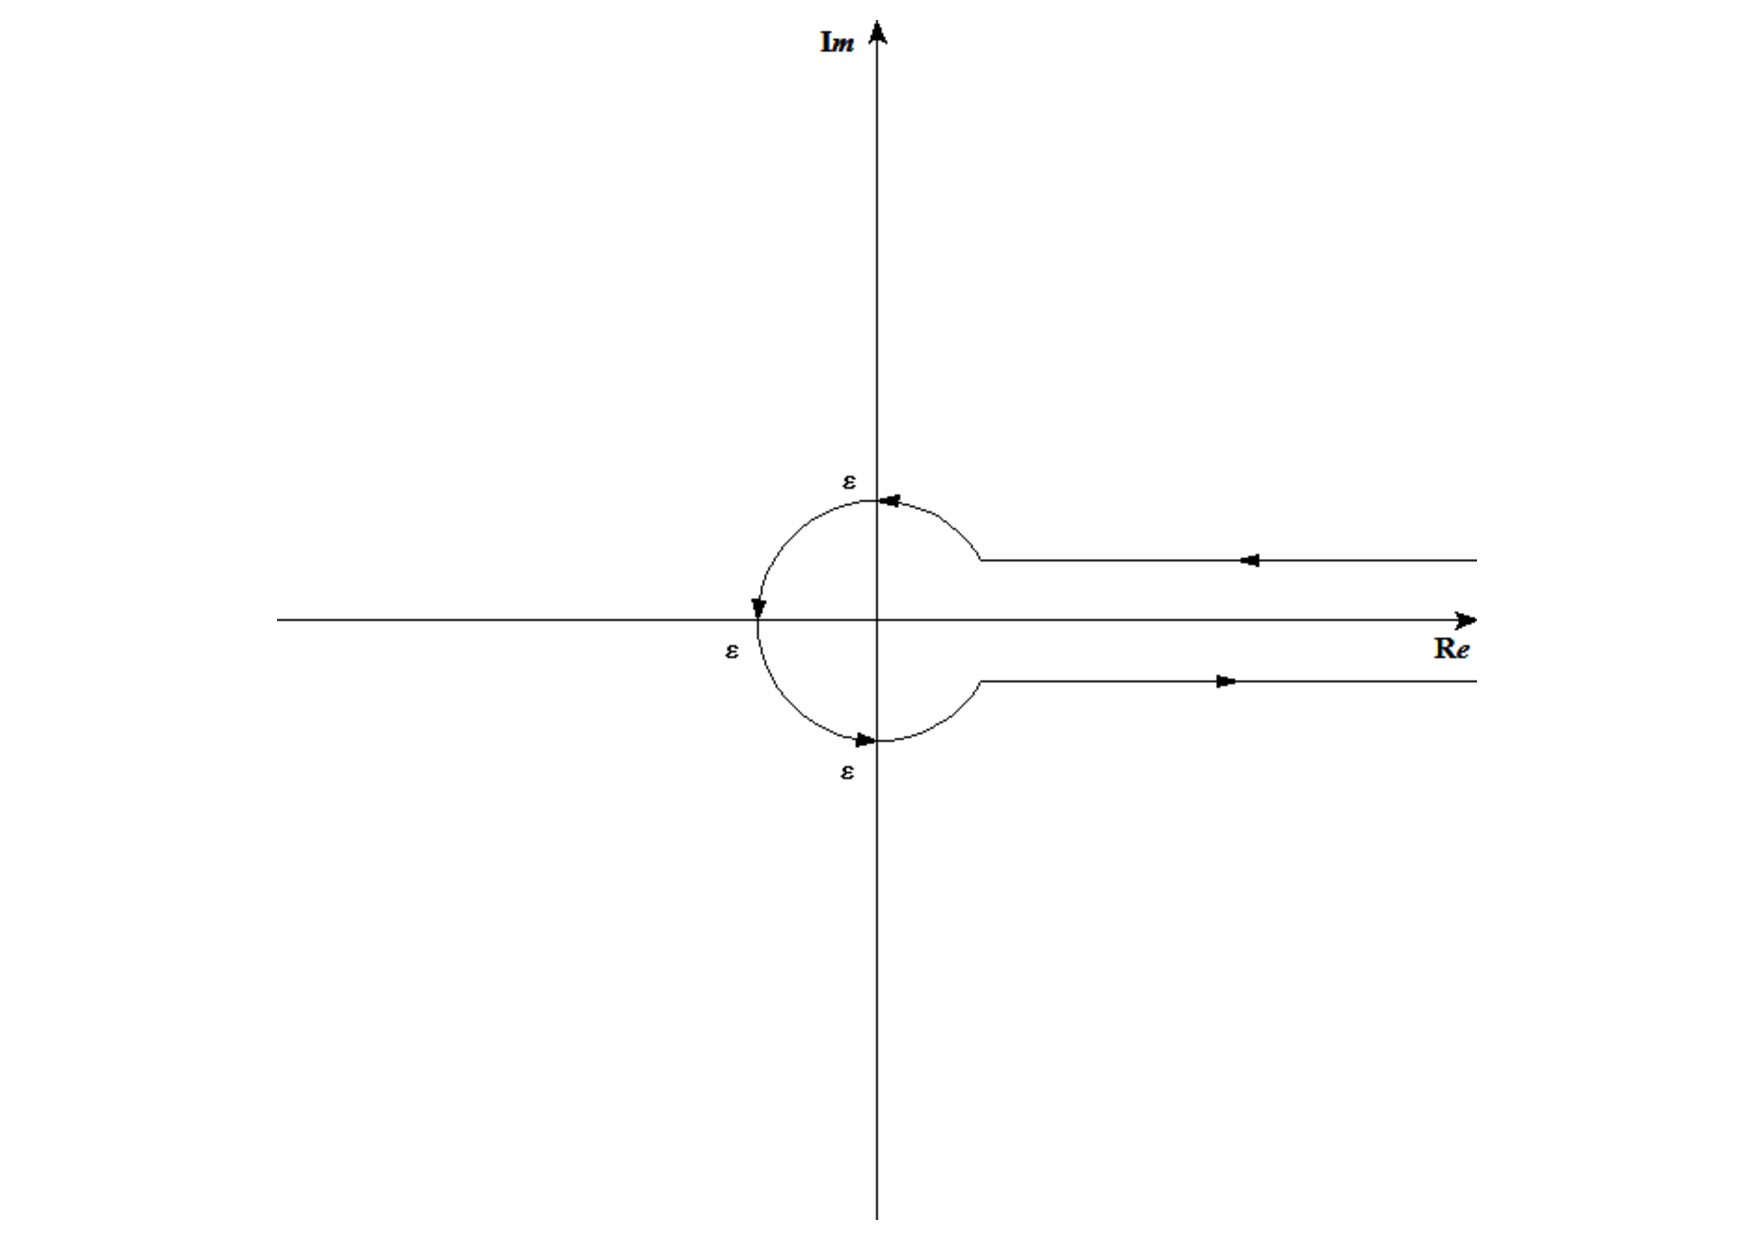
\includegraphics[width=50mm]{zetamura2.pdf}
\end{center}
\end{wrapfigure}
ここで以下の積分を考える.
\[
\int_{\infty}^{\infty} \frac{(-z)^{s-1}dz}{e^z-1}
\]
積分経路は,実軸よりわずかに上を通って$\infty$から0へと向かい, 0の周りを回ったのち,実軸のわずかに下を通って0から$\infty$へと向かう.\\
ただし, $(-z)^{s-1}=e^{(s-1)\log(-z)}$とし, $\log z$は主枝を選ぶ.\\

この積分を
\begin{align}
\int_{\infty}^\epsilon \frac{(-z)^{s-1}dz}{e^z-1}+\int_{|z|=\epsilon} \frac{(-z)^{s-1}dz}{e^z-1}+\int_\epsilon^{\infty} \frac{(-z)^{s-1}dz}{e^z-1}\label{eq:2}
\end{align}
と分割すると,中央の項は$Re(s)>1$において$\epsilon\to0$のとき0に近づく.\\
なぜなら, $|z|=\epsilon$のとき$|e^z-1|>1-e^{-\epsilon}>0$より$\frac{1}{|e^z-1|}<\frac{1}{1-e^{-\epsilon}}$であるから
\begin{eqnarray*}
\left|\frac{(-z)^{s-1}}{e^z-1}\right| \le \frac{\epsilon^{Re(s)-1}}{1-e^{-\epsilon}}
\end{eqnarray*}
であり, $\epsilon\to0$のとき
\begin{eqnarray*}
\left|\int_{|z|=\epsilon} \frac{(-z)^{s-1}dz}{e^z-1}\right| &\le& 2\pi\epsilon \frac{\epsilon^{Re(s)-1}}{1-e^{-\epsilon}}\\
&=& 2\pi\frac{\epsilon}{1-e^{-\epsilon}}\epsilon^{Re(s)-1}\to0
\end{eqnarray*}
となるからである.\\
残った2つの項をまとめると
\begin{eqnarray*}
\lim_{\epsilon \to 0}\left(\int_{\infty}^\epsilon \frac{(-z)^{s-1}dz}{e^z-1}+\int_\epsilon^{\infty} \frac{(-z)^{s-1}dz}{e^z-1}\right) &=& \lim_{\epsilon \to 0}\left(\int_{\infty}^\epsilon \frac{e^{(s-1)(\log z-i\pi)}dz}{e^z-1}+\int_\epsilon^{\infty} \frac{e^{(s-1)(\log z+i\pi)}dz}{e^z-1}\right)\\
&=& (e^{-\pi si}-e^{\pi si}) \int_0^\infty \frac{z^{s-1}dz}{e^z-1}\\
&=& -2i\sin{\pi s}\int_0^\infty \frac{z^{s-1}dz}{e^z-1}
\end{eqnarray*}
これを式(\ref{eq:1})と合わせれば次を得る.
\[
-2i\sin{\pi s}\,\Pi(s-1)\zeta(s)=\int_\infty^\infty \frac{(-z)^{s-1}dz}{e^z-1}
\]
右辺の積分は全てのsに対して収束し,正則である.\\
\[
\Pi(s-1)\Pi(-s)=\frac{\pi}{\sin{\pi s}}
\]
を用いれば
\begin{align}
\zeta(s)=-\frac{\Pi(-s)}{2\pi i}\int_{\infty}^{\infty} \frac{(-z)^{s-1}dz}{e^z-1}\label{eq:3}
\end{align}
となる.この式は複素平面上における$s=1$を除いて解析的な関数$\zeta(s)$を定義し, $Re(s)>1$において$\sum n^{-s}$と一致する.\\

\Section{\S 3.関数等式}
\begin{wrapfigure}[8]{r}{50mm}
\vspace{-2\baselineskip}
\begin{center}
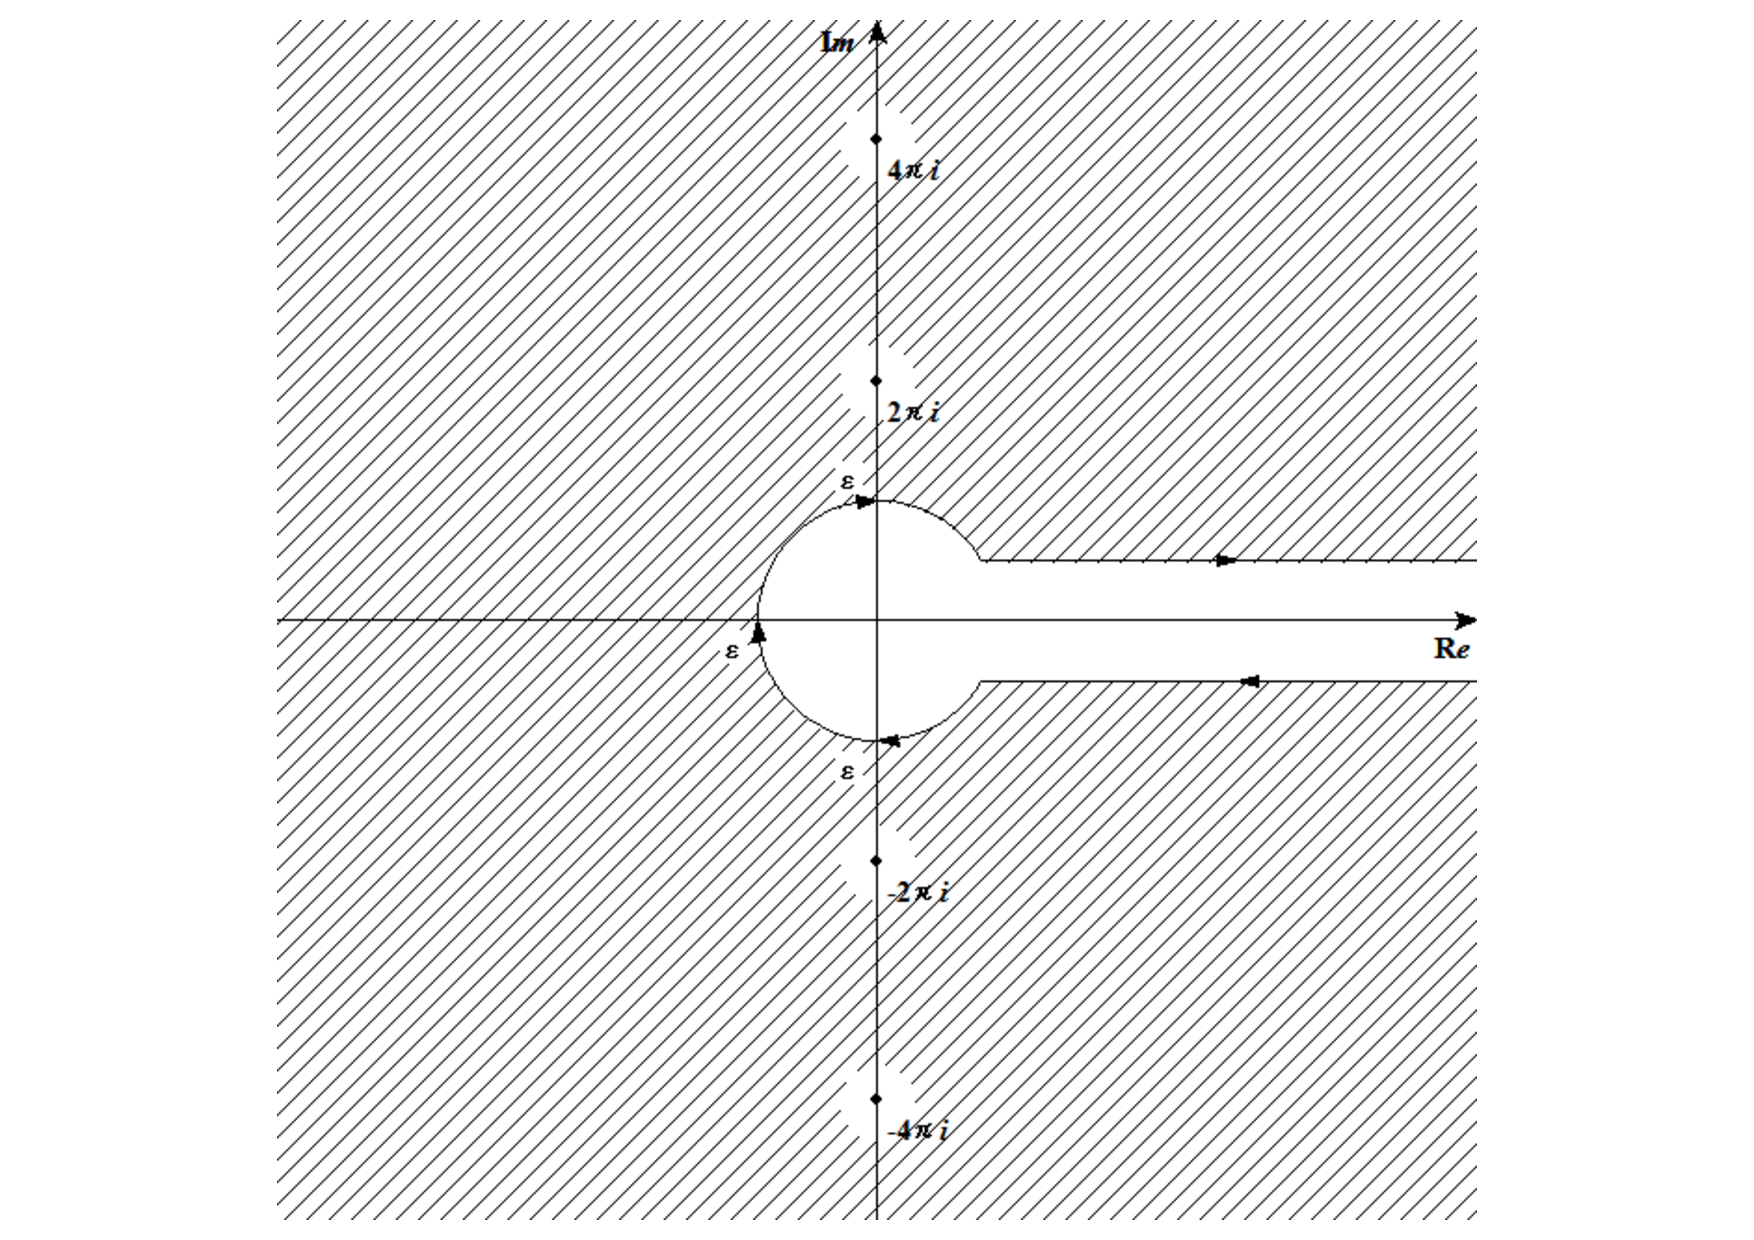
\includegraphics[width=50mm]{zetamura3.pdf}
\end{center}
\end{wrapfigure}
式(\ref{eq:3})において,積分経路を逆向きにとることで0以外の1位の極$z=2n\pi i\,(n=\pm1,\pm2,\ldots)$を含む領域に沿った積分とすることができる.値は$-1$倍になる事に注意して
\begin{eqnarray*}
\lim_{z\to 2n\pi i}(z-2n\pi i)\frac{(-z)^{s-1}}{e^z-1} &=& \lim_{z\to 2n\pi i}\frac{z-2n\pi i}{e^z-e^{2n\pi i}}(-z)^{s-1}\\
&=& (-2n\pi i)^{s-1}
\end{eqnarray*}
より
\begin{eqnarray}
\zeta(s) &=& \Pi(-s)\sum_{n=1}^\infty ((-2n\pi i)^{s-1}+(2n\pi i)^{s-1})\nonumber\\
&=& \Pi(-s)(2\pi)^{s-1}\left(i^{s-1}+(-i)^{s-1}\right)\sum_{n=1}^\infty n^{s-1}\nonumber\\
&=& \Pi(-s)(2\pi)^{s-1}2\sin\left(\frac{s\pi}{2}\right)\zeta(1-s)\label{eq:4}
\end{eqnarray}
が得られる.

\Section{\S 4.$\zeta(s)$の値}
さて, $\zeta(s)$の値をいくつか求めてみよう.\\
$s=-n\,(n\in\mathbb{N})$のとき,式(\ref{eq:3})より
\[
\zeta(-n) = -\frac{\Pi(n)}{2\pi i}\int_\infty^\infty \frac{(-z)^{-n-1}dz}{e^z-1}
\]
式(\ref{eq:2})と同様に分割すると,今度は第1項と第3項が打ち消し合い第2項のみが残るので
\begin{eqnarray*}
\zeta(-n) &=& -\frac{\Pi(n)}{2\pi i}\int_{|z|=\epsilon} \frac{(-z)^{-n-1}dz}{e^z-1}\\
&=& (-1)^n\frac{\Pi(n)}{2\pi i}\int_{|z|=\epsilon}\frac{z}{e^z-1}z^{-n-2}dz\\
&=& (-1)^n\frac{\Pi(n)}{2\pi i}\int_{|z|=\epsilon} \left(\sum_{m=0}^\infty \frac{B_m z^m}{m!}\right)z^{-n-2}dz\\
&=& (-1)^n \Pi(n)\sum_{m=1}^\infty \frac{B_m}{m!} \frac{1}{2\pi i}\int_{|z|=\epsilon} z^{m-n-2}dz\\
&=& (-1)^n n!\frac{B_{n+1}}{(n+1)!}\\
&=& (-1)^n \frac{B_{n+1}}{n+1}
\end{eqnarray*}

また, $n$を$2n-1$とすれば
\[
\zeta(-(2n-1))=(-1)^{2n-1}\frac{B_{2n}}{2n}
\]
となるが,関数等式(\ref{eq:4})を用いると
\[
\zeta(-(2n-1))=\Pi(2n-1)(2\pi)^{-2n}2\sin\left(\frac{-(2n-1)\pi}{2}\right)\zeta(2n)
\]
である.従って
\[
\zeta(2n)=(-1)^{n+1}\frac{(2\pi)^{2n}B_{2n}}{2(2n)!}
\]
を得る.\\
これらより最初に述べた式
\begin{eqnarray*}
\zeta(2)=\frac{\pi^2}{6}, \zeta(4)=\frac{\pi^4}{90}, \zeta(6)=\frac{\pi^6}{945}\\
\zeta(0)=-\frac{1}{2}, \zeta(-1)=-\frac{1}{12}
\end{eqnarray*}
等が求まるのである.

\Section{\S 5.解析接続の意味}
ゼータ関数を解析接続することで通常の和の意味では発散してしまう値を求めたわけでだが,これはどういう意味をもつのであろうか.\\
実は,例えば$Re s>-3$なるすべての複素数に対して
\[
\zeta(s)=\lim_{N\to\infty}\left\{\sum_{n=1}^N n^{-s}-\left(\frac{1}{1-s}N^{1-s}+\frac{1}{2}N^{-s}-\frac{s}{12}N^{-s-1}\right)\right\}
\]
となっている.\\
オイラーマクローリンの公式によれば
\[
\sum_{n=1}^N n^{-s}=\frac{1}{1-s}N^{1-s}+\frac{1}{2}N^{-s}-\frac{s}{12}N^{-s-1}+o(N^{-s-2})
\]
であるから,これと比較すればゼータ関数の解析接続は$\sum_{n=1}^N n^{-s}$の発散する部分を取り除いた和を求める,いわゆる繰り込みを行っているのである.従って最初に述べた
\begin{eqnarray*}
\zeta(0)=1+1+\cdots &=& -\frac{1}{2}\\
\zeta(-1)=1+2+\cdots &=& -\frac{1}{12}
\end{eqnarray*}
は正確ではなく,あくまで$\sum_{n=1}^\infty n^{-s}$を解析接続した関数$\zeta(s)$が$\zeta(0)=-\frac{1}{2},\zeta(-1)=-\frac{1}{12}$であると解釈する方が良いだろう.
\Section{参考文献}
\begin{description}
\item{[Harold]} ハロルド, M, E. 鈴木治郎訳(2012)『明解 ゼータ関数とリーマン予想』講談社
\item{[Kurokawa]} 黒川信重(2014)『ゼータの冒険と進化』現代数学社
\item{[Riemann]} Riemann, B. (1859). Ueber die anzahl der primzahlen unter einer gegebenen gr\"{o}sse. \textit{Monatsberichte der Berliner Akademie}, \textit{November 1859}, 671-680.
\end{description}

%\begin{thebibliography}{9}
%\bibitem{Harold}
%ハロルド, M, E. 鈴木治郎訳(2012)『明解 ゼータ関数とリーマン予想』講談社
%\bibitem{Kurokawa}
%黒川信重(2014)『ゼータの冒険と進化』現代数学社
%\bibitem{Riemann}
%Riemann, B. (1859). Ueber die anzahl der primzahlen unter einer gegebenen gr\"{o}sse. \textit{Monatsberichte der Berliner Akademie}, \textit{November 1859}, 671-680.
%\end{thebibliography}
